% H = 128 vs H = 256 for both models.
% Numbers from evaluations/fa_{unconditional,conditional}_H{128,256}/{metrics,tree_comparison,mode_mixing}.json

\section{Results: more heads, $H=256$}\label{sec:res_H256}
Both models were retrained with $H=256$ heads, the value suggested by the rank argument of \S\ref{sec:rank}
($H\ge179$). All other settings were identical (configs \texttt{fa\_unconditional\_H256.json},
\texttt{fa\_conditional\_H256.json}; runs \texttt{fa\_*\_H256}).

\subsection{Summary table}
\begin{center}\footnotesize
\begin{tabular}{lcccc}
\toprule
 & \multicolumn{2}{c}{unconditioned} & \multicolumn{2}{c}{conditioned}\\
 & $H=128$ & $H=256$ & $H=128$ & $H=256$\\
\midrule
parameters & 0.54\,M & 1.09\,M & 2.12\,M & 4.19\,M\\
best epoch (stopped at) & 57 (60) & 36 (45) & 38 (47) & 10 (18)\\
validation pseudo-NLL / site & 0.949 & \textbf{0.946} & \textbf{0.873} & 0.888\\
\midrule
\multicolumn{5}{l}{\emph{parameters vs the ground truth (contact entries, zero-sum gauge)}}\\
$r_J$ (vs average of clades / matched clade) & 0.691 & \textbf{0.771} & 0.640 & \textbf{0.664}\\
slope of $J$ & 0.57 & \textbf{0.62} & \textbf{0.40} & 0.37\\
$r_h$ & \textbf{0.922} & 0.898 & \textbf{0.871} & 0.791\\
$r(\Delta J)$ family / subfamily / clade & -- & -- & 0.34/0.21/0.11 & 0.38/0.24/0.12\\
$r(\Delta h)$ family / subfamily / clade & -- & -- & 0.58/0.50/0.33 & 0.51/0.42/0.26\\
long-range contact precision & 1.00 & 1.00 & 1.00 & 1.00\\
\midrule
\multicolumn{5}{l}{\emph{generated sequences vs held-out test sequences}}\\
family shares (no tag) & 22/12/66\% & 11/13/76\% & 33/21/46\% & \textbf{28/31/41\%}\\
pooled $r_C$ (oracle 0.994) & \textbf{0.895} & 0.855 & \textbf{0.954} & 0.919\\
pooled $r_C$ after rebalancing & 0.949 & \textbf{0.952} & -- & --\\
per-clade $r_C$ (oracle 0.83) & -- & -- & \textbf{0.758} & 0.704\\
family-tag $r_C$ (mean) & -- & -- & 0.849 & \textbf{0.865}\\
per-clade FD in PCA space (oracle 0.02) & -- & -- & \textbf{0.39} & 0.62\\
FD assignment accuracy & -- & -- & \textbf{17/18} & 16/18\\
pairwise $\bar D_{GG}$ (test value) & 0.740 (0.803) & 0.716 (0.803) & 0.637 (0.663) & 0.633 (0.663)\\
mean $d_{NN}$ to train (test value 0.378) & 0.398 & 0.384 & 0.370 & 0.374\\
copies of training sequences & 0 & 0 & 0 & 0\\
\bottomrule
\end{tabular}
\end{center}

\subsection{Unconditioned model: better couplings, worse family weights}
With $H=256$ the learned couplings get closer to the truth ($r_J$ with the average of the clades $0.69\to0.77$,
slope $0.57\to0.62$; with the root $0.65\to0.73$). The statistics \emph{inside} each family improve (rebalanced
pooled $r_C$ 0.949 $\to$ 0.952). But the family weights get \emph{worse}: 11/13/76\% instead of 22/12/66\%. So the
pooled statistics, which include the weights, degrade ($r_C$ $0.895\to0.855$). The mixing check (\texttt{s08})
confirms again that this is the learned distribution, not the sampler: all starts converge to $\approx10/12/78\%$.
The energy/entropy decomposition \eqref{eq:freeenergy} gives an energy advantage of 13.3--13.5 for F2, compensated
by an entropy deficit of 11.6--11.8, a residual of $\approx1.8$ nats instead of 1.1--1.6.

This is a clean illustration of the pseudo-likelihood blind spot: \textbf{more capacity improves exactly what PL
measures} (each site given the others, $J$ and within-family statistics) \textbf{and does nothing for what PL
cannot see} (the relative weights of the families). A small, uncontrolled drift of the energy/entropy balance then
moves the weights further away.

\begin{figure}[H]
\centering
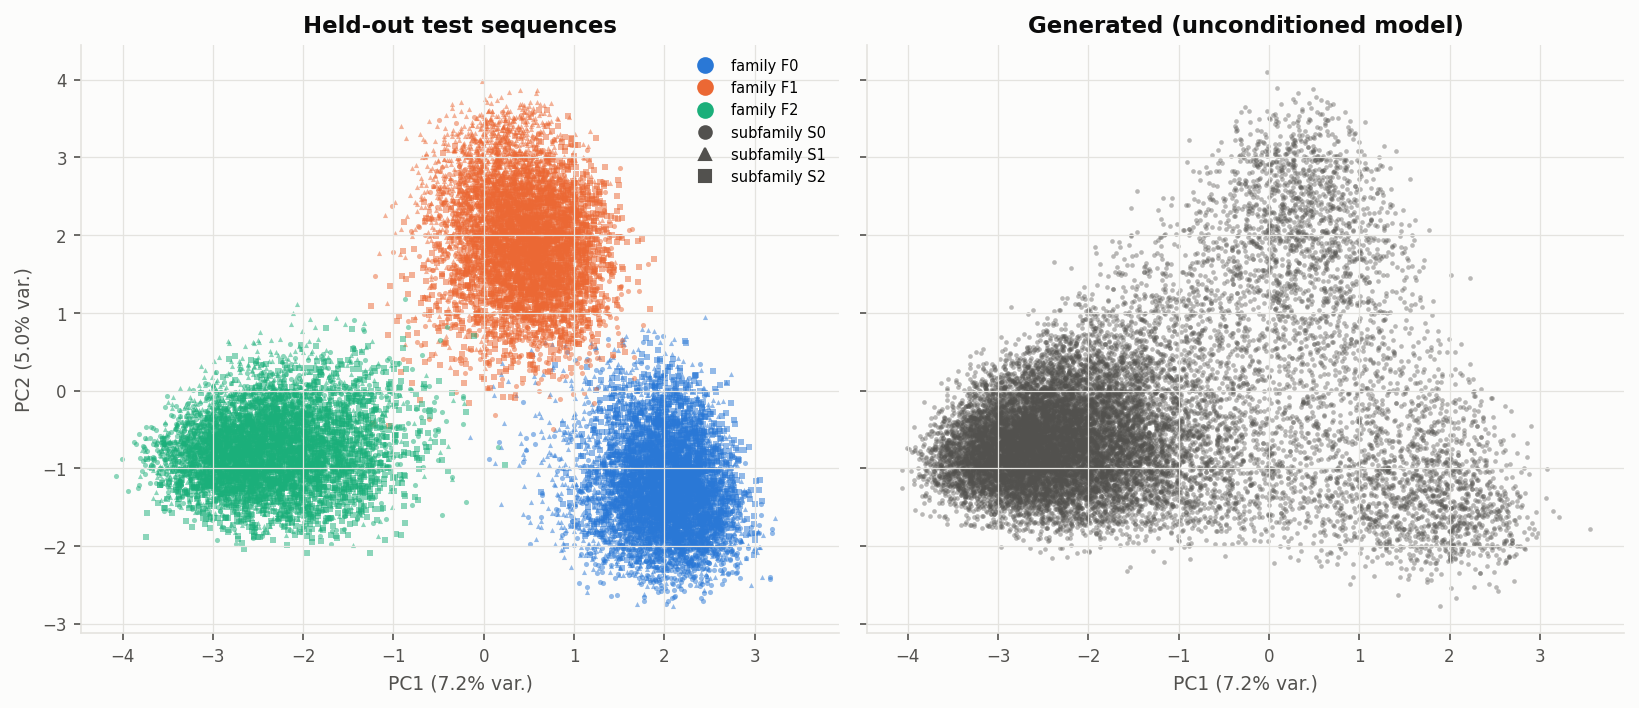
\includegraphics[width=0.85\linewidth]{models/fa_unconditional_H256/pca_generated_vs_test.png}
\caption{Unconditioned model with $H=256$: generated sequences on the reference PCA (right). F2 (bottom left) now
holds 76\% of the samples.}
\end{figure}

\subsection{Conditioned model: more heads did not help here}
The conditioned model with $H=256$ is \emph{worse} on most sequence metrics (per-clade $r_C$ $0.76\to0.70$, FD
$0.39\to0.62$), although its couplings are slightly better ($r_J$ $0.64\to0.66$, $r(\Delta J)$ slightly up at every
level). The reason is visible in the training curve. The validation loss is best at epoch 10 and does not improve afterwards, so
early stopping ended training at epoch 18. With twice the heads, the label tables hold twice as many parameters
(3.1\,M instead of 1.6\,M) under the same penalty $\lambda_{\text{label}}$. They start fitting noise within a few
epochs, before the fields have converged. The fields are indeed the component that got worse ($r_h$ $0.87\to0.79$,
$r(\Delta h)$ down at every level), and the fields are what carries the clade identity (\S\ref{sec:res_cond}).
Family-level behaviour, by contrast, improved: family tags are slightly better ($r_C$ 0.849 $\to$ 0.865) and the
no-tag family weights are closer to uniform (28/31/41\%). The mixing check confirms these weights (all starts
converge to $\approx28/31/41\%$), and the energy/entropy residual shrinks to 0.2--0.4 nats (energy terms $-9.1$ and
$-9.6$, entropy terms $+8.7$ and $+9.4$ for F0 and F1 relative to F2).

\begin{figure}[H]
\centering
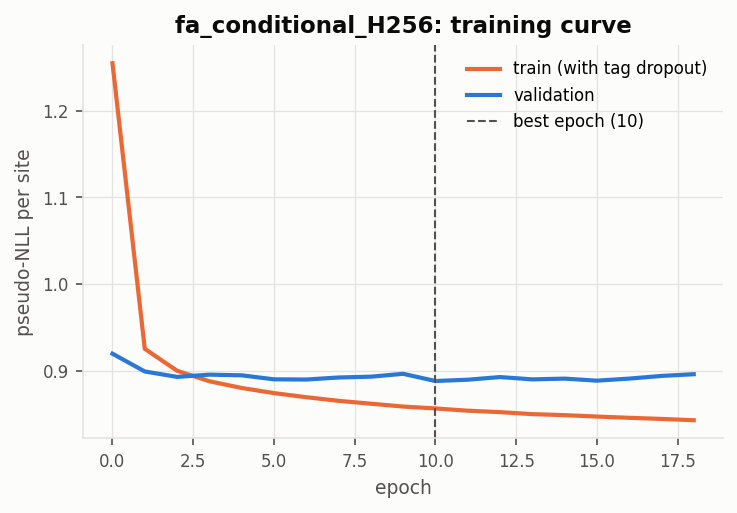
\includegraphics[width=0.49\linewidth]{models/fa_conditional_H256/training_curve.png}\hfill
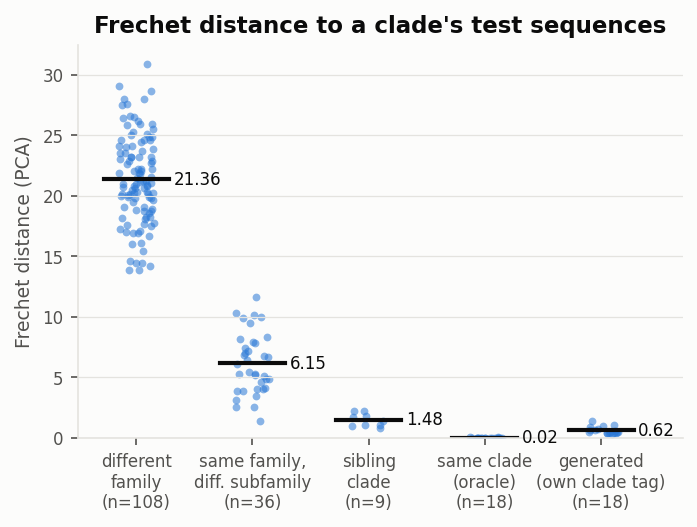
\includegraphics[width=0.49\linewidth]{models/fa_conditional_H256/frechet_ladder.png}
\caption{Conditioned model with $H=256$. Left: training curve (best epoch 10; compare the $H=128$ curve, best epoch 38).
Right: FD ladder; the generated clades (right-most column, mean 0.62) sit farther from their own clade than at
$H=128$ (0.39), still below the sibling clade (1.48).}
\end{figure}

\begin{keybox}{Conclusion on $H$}
\begin{itemize}[nosep]
\item $H=256$ recovers the couplings better in both models, as the rank argument predicts.
\item For the unconditioned model this does not translate into better samples, because its main error (family
      weights) is invisible to pseudo-likelihood and got worse.
\item For the conditioned model, the doubled label tables over-fit quickly with the current
      $\lambda_{\text{label}}=10^{-4}$, and early stopping cuts training before the fields are learned.
      $H=256$ therefore needs a stronger label penalty (or a smaller learning rate / more data per clade). As it
      stands, \textbf{the best generator is still the conditioned model with $H=128$}.
\end{itemize}
\end{keybox}
